\documentclass[11pt]{article}

\usepackage[margin=1in]{geometry}
\usepackage[T1]{fontenc}
\usepackage[utf8]{inputenc}
\usepackage{lmodern}
\usepackage{microtype}
\usepackage{amsmath,amssymb,amsthm,bm}
\usepackage{booktabs}
\usepackage{graphicx}
\usepackage{float}
\usepackage{multirow}
\usepackage{hyperref}
\usepackage[numbers]{natbib}
\usepackage{setspace}
\usepackage{caption}
\usepackage{subcaption}
\usepackage{threeparttable}

\hypersetup{colorlinks=true,citecolor=blue,linkcolor=blue,urlcolor=blue}
\setstretch{1.12}
\setlength{\parindent}{15pt}
\setlength{\parskip}{0pt}
\captionsetup{
    font=small,
    labelfont=bf,
    justification=justified,
    singlelinecheck=false
}
\captionsetup[subfigure]{font=small}
\numberwithin{equation}{section}
\allowdisplaybreaks[2]

\theoremstyle{plain}
\newtheorem{proposition}{Proposition}[section]

\makeatletter
\renewcommand{\maketitle}{%
  \begin{center}
    {\LARGE \bfseries \@title \par}
    \vspace{1em}
    {\normalsize \@date \par}
  \end{center}
  \vspace{1em}
}
\makeatother

\renewenvironment{abstract}
  {\begin{center}\bfseries Abstract\end{center}\begin{quote}\small}
  {\end{quote}\vspace{1em}}

\title{Do Prediction Markets Match Option Prices?\\ Bitcoin Threshold Evidence from Binance and Polymarket}
\author{}
\date{March 2026}

\begin{document}
\maketitle

\begin{abstract}
We compare Polymarket Yes prices for Bitcoin ``above $K$ by $T$'' events to a benchmark from matched Binance calls. Each hour, Black--Scholes implied volatility is backed out from the observed call; the discounted binary value $P_{fair,t}$ is set against the Polymarket price $P_{poly,t}$, with gap $D_t=P_{poly,t}-P_{fair,t}$, using public archives at hourly alignment. The main September~2023 contract yields mean $D$ of $0.0558$ over $214$ hours ($p<10^{-9}$; 95\% correlation-robust interval $[0.0228,\,0.0889]$). Pooling three markets gives mean $0.0633$ over $287$ hours with similar evidence. Polymarket exceeds the option-implied level on average in this sample; conclusions depend on the model and the narrow contract set.
\end{abstract}

\section{Introduction}
If a contract pays \$1 when Bitcoin finishes above a fixed level on a fixed date, finance textbooks price that payoff from listed options on the same asset. The idea is not to guess tomorrow's weather from history, but to read off what option prices already say about the chance of finishing above the strike. Here we ask a narrow, concrete question: for matched strike and date, does Polymarket's Yes price, on average, match the level implied by Binance options?

Once strikes and expiries line up, agreement would show up as an average $D_t$ near zero. A steady positive or negative average means one venue is usually higher or lower than the other. We infer volatility from the observed call each hour, turn it into the implied fair level for the binary payoff, and test whether the average gap is zero using (i) the usual $t$-test, (ii) an interval that allows hours to be correlated \citep{newey1987}, and (iii) a bootstrap that keeps chunks of consecutive hours together \citep{casella2002}. Data are Binance's public option and spot files and Polymarket trades, all placed on the same Yes-price scale.

In the 2023 window we study, the average gap is positive: roughly $5.6$ percentage points for the headline contract and about $6.3$ points when three contracts are stacked.

\section{Data}
\subsection{What is being compared?}
Each Polymarket Yes share pays \$1 if Bitcoin is above strike $K$ when the contract closes. The fair value of that payoff can be tied to a European call with the same strike and maturity: once you know how volatile the market looks, the model pins down a price for ``finish above $K$.'' Section~\ref{sec:model} states the standard Black--Scholes link in symbols; here the takeaway is that we compare apples to apples---same event, two prices.

\subsection{Sources and sample}
Everything is drawn from public feeds: Binance option end-of-hour summaries (\texttt{EOHSummary}) and hourly spot bars \citep{binancepublicdata}, plus Polymarket trades (and hourly prices when available) \citep{polymarketdocs}. The main illustration is ``BTC above \$27{,}000 at end of September?'' next to call \texttt{BTC-230929-27000-C}. Two August~2023 thresholds are added for a small pooled check. After cleaning and alignment there are $214$ hours for the flagship case and $287$ pooled.

\subsection{Symbols at a glance}
\begin{center}
\begin{tabular}{ll}
\toprule
Symbol & Plain meaning \\
\midrule
$C_{mkt,t}$ & Observed Binance call price (mid of bid and ask when both exist) \\
$S_t$ & Bitcoin spot in the same hour \\
$K$ & Strike shared by the two contracts \\
$\tau_t$, $\tau_t^{(c)}$ & Time left until Polymarket settles / until the option expires (in years, 365-day year) \\
$P_{poly,t}$ & Polymarket price as a Yes probability in $[0,1]$ \\
$P_{fair,t}$ & Fair level implied from the option (Section~\ref{sec:model}) \\
$D_t$ & Gap: Polymarket minus fair, $P_{poly,t}-P_{fair,t}$ \\
\bottomrule
\end{tabular}
\end{center}
Yes and No trades are converted to the same scale: a Yes at price $p$ counts as $p$, a No at $p$ counts as $1-p$.

\subsection{Alignment}
All series use the same hour stamp. For each Binance hour we take the latest Polymarket observation on or before that time. Hours with almost no time left to expiry are removed so the volatility step stays well behaved.

\section{How the comparison is built}\label{sec:model}
\subsection{From option price to fair Yes level}
Under Black--Scholes \citep{black1973}, a European call is priced by $C_{BS}=S_t\Phi(d_1)-Ke^{-r\tau}\Phi(d_2)$ with the usual $d_1,d_2$. The model also implies a discounted probability of finishing above $K$, which we use as the benchmark:
\[
P_{fair,t}(\sigma)=e^{-r\tau_t}\Phi(d_{2,t}(\sigma)).
\]
Proposition~\ref{prop:digital-price} derives this step.

\subsection{Backing out volatility each hour}
Each hour, $\hat{\sigma}_t$ is the volatility that makes the model call price match the observed quote (Newton iteration; sensitivity of the call to volatility is in Proposition~\ref{prop:vega-formula}). We keep only solutions where the fit is tight and the sensitivity is not tiny. Then $P_{fair,t}=e^{-r\tau_t}\Phi(d_2(\hat{\sigma}_t))$.

\subsection{How uncertain is the benchmark? (shading in figures)}
$P_{fair,t}$ moves when the call quote moves. We translate noise in the quote into a standard error for $P_{fair,t}$ using standard first-order logic (sometimes called the delta method; details in Propositions~\ref{prop:digital-sensitivity}--\ref{prop:iv-delta}). Quote uncertainty is proxied by half the hourly high--low range on the option, with a small floor. Figures shade $P_{fair,t}\pm 1.96\,SE(P_{fair,t})$ to show how tight the fitted benchmark is \emph{given the data}; it is not a market forecast interval.

\subsection{Testing whether the average gap is zero}
We care about the long-run average of $D_t=P_{poly,t}-P_{fair,t}$. Besides the textbook one-sample $t$-test, we report an interval that allows successive hours to be correlated \citep{newey1987} and a bootstrap that resamples blocks of hours together. Proposition~\ref{prop:tick-noise} notes that Polymarket prices live on a tick grid; that detail is secondary for the average-gap tests.

\subsection{Does the gap linger?}
We summarize persistence with a simple AR(1) in $D_t$ and a unit-root check (augmented Dickey--Fuller) \citep{dickey1979}.

\section{Results}
\subsection{Main example}
We focus on ``BTC above \$27{,}000 at end of September?'' with Binance call \texttt{BTC-230929-27000-C}. There are $214$ matched hours. Average levels over the window:
\[
\overline{C_{mkt}} = 253.446,
\qquad
\overline{S_t} = 26{,}664.80,
\qquad
\overline{P_{poly}} = 0.4043,
\qquad
\overline{P_{fair}} = 0.3484.
\]
Polymarket is higher on average: $\bar{D}=0.0558$ with spread $s_D=0.1264$, i.e.\ about $5.6$ percentage points on the probability scale.

Table~\ref{tab:main} collects the formal checks.

\begin{table}[H]
\centering
\caption{Main example: BTC above \$27{,}000 at end of September}
\label{tab:main}
\begin{threeparttable}
\begin{tabular}{lc}
\toprule
Quantity & Value \\
\midrule
Hours $n$ & 214 \\
Average gap $\bar{D}$ & 0.0558*** \\
Spread of gaps $s_D$ & 0.1264 \\
$t$-statistic (gap $=0$) & 6.46 \\
Two-sided $p$ value & $6.86 \times 10^{-10}$ \\
95\% interval, correlation-robust & [0.0228, 0.0889] \\
95\% interval, block bootstrap & [0.0212, 0.0911] \\
Typical uncertainty in fair level (mean $SE$) & 0.0458 \\
\bottomrule
\end{tabular}
\begin{tablenotes}[flushleft]
\footnotesize
\item \textit{Notes.} Stars mark significance of the average gap being different from zero: * 10\%, ** 5\%, *** 1\%.
\end{tablenotes}
\end{threeparttable}
\end{table}

All three intervals sit strictly above zero.

Figure~\ref{fig:main_ts} plots Polymarket against the fair level. The gray band is $\pm 1.96$ standard errors around the fitted fair value (Section~\ref{sec:model}). The lower panel is the gap $D_t$.

\begin{figure}[H]
\centering
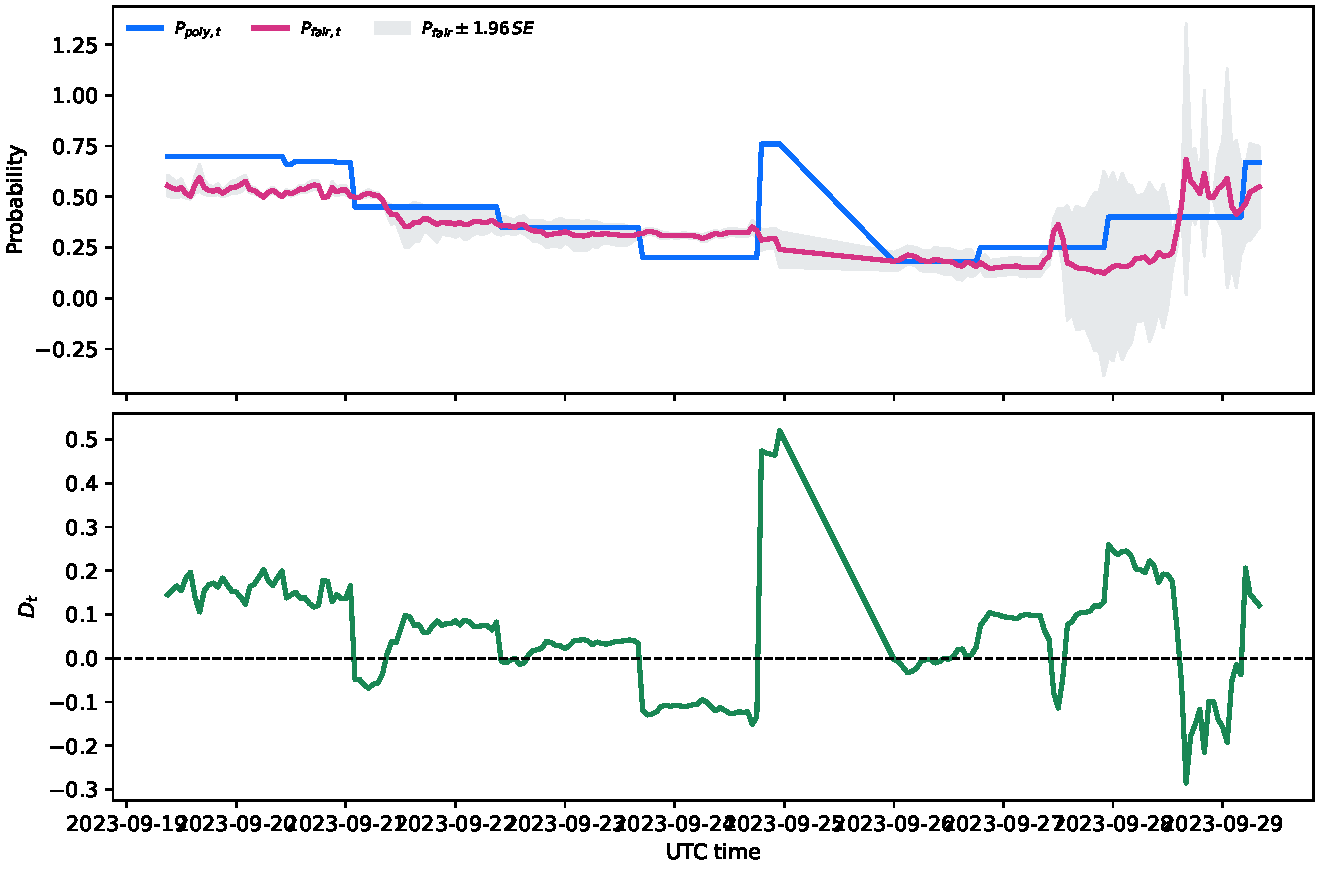
\includegraphics[width=0.84\textwidth]{figures/main_timeseries.pdf}
\caption{Main example. \emph{Top:} Polymarket Yes (blue), fair level from the option (pink), and a light band for estimation noise around the fair level. \emph{Bottom:} gap $D_t=$ Polymarket minus fair.}
\label{fig:main_ts}
\end{figure}

\subsection{Three contracts together}
Combining three matched contracts yields $n=287$ hours, average gap $0.0633$, correlation-robust 95\% interval $[0.0327,\,0.0940]$, bootstrap interval $[0.0308,\,0.0950]$, and $t=8.24$ ($p=6.26\times 10^{-15}$). The September result is not a one-off.

Figure~\ref{fig:pooled_panels} shows how gaps are distributed when markets are stacked, and how the average gap compares contract by contract.

\begin{figure}[H]
\centering
\begin{subfigure}[t]{0.47\textwidth}
\centering
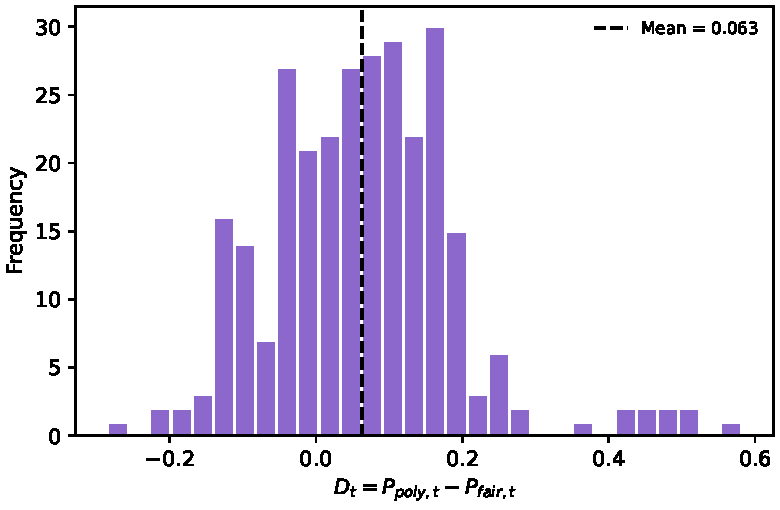
\includegraphics[width=\textwidth]{figures/pooled_histogram.pdf}
\caption{Histogram of all gaps in the pooled sample.}
\label{fig:pooled_hist}
\end{subfigure}
\hfill
\begin{subfigure}[t]{0.49\textwidth}
\centering
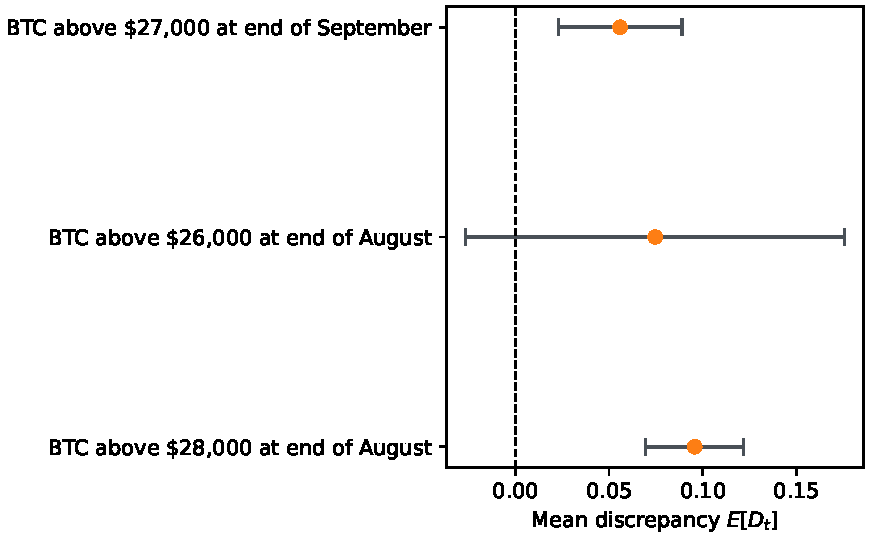
\includegraphics[width=\textwidth]{figures/market_means.pdf}
\caption{Average gap by market (dots) with 95\% correlation-robust intervals.}
\label{fig:market_means}
\end{subfigure}
\caption{Pooled sample. \subref{fig:pooled_hist}: spread of $D_t$. \subref{fig:market_means}: average gap per market.}
\label{fig:pooled_panels}
\end{figure}

\begin{table}[H]
\centering
\caption{Each contract and the pooled row}
\label{tab:markets}
\begin{threeparttable}
\begin{tabular}{lccc}
\toprule
Market & Hours $n$ & Avg.\ gap & 95\% interval \\
\midrule
BTC above \$28{,}000 at end of August & 37 & 0.0957*** & [0.0695, 0.1218] \\
BTC above \$26{,}000 at end of August & 36 & 0.0745** & [-0.0267, 0.1758] \\
BTC above \$27{,}000 at end of September & 214 & 0.0558*** & [0.0228, 0.0889] \\
Pooled & 287 & 0.0633*** & [0.0327, 0.0940] \\
\bottomrule
\end{tabular}
\begin{tablenotes}[flushleft]
\footnotesize
\item \textit{Notes.} Stars as in Table~\ref{tab:main}.
\end{tablenotes}
\end{threeparttable}
\end{table}

Every point estimate is positive; the August \$26{,}000 case is wide because prices spend much of the sample near certainty.

\subsection{Does the gap fade quickly?}
For the main contract, a unit-root test suggests $D_t$ is not a pure random walk ($p\approx 0.004$). A simple AR(1) with coefficient near $0.85$ implies gaps decay slowly (half-life on the order of a few hours): they linger for a while but do not drift without bound.

\section{Discussion}
The fair level comes from a textbook model---lognormal prices, one volatility number per hour---so it is a reference line, not ground truth. Polymarket and Binance also settle trades under different rules. Only three contracts enter the pooled row, so readers should treat the numbers as a case study, not a verdict on all prediction markets.

\section{Conclusion}
For matched ``Bitcoin above $K$'' events in 2023, Polymarket Yes prices in our sample averaged several percentage points above the levels backed out from Binance options in the same hours, and that average difference is clearly different from zero under both standard and correlation-aware tests. Wider contract coverage and richer models would be the next steps.

\appendix

\section{Analytical Derivations}

\begin{proposition}[Risk-neutral valuation of the binary payoff]
\label{prop:digital-price}
Let $S$ follow Black--Scholes dynamics under the risk-neutral measure,
\[
\frac{dS_t}{S_t}=r\,dt+\sigma\,dW_t^{\mathbb{Q}},
\]
with constant $r$ and $\sigma$. Consider the unit payoff $\mathbf{1}\{S_T>K\}$ at maturity $T$. Then its time-$t$ value is
\[
P_{fair,t}=e^{-r\tau}\Phi(d_2),
\qquad
\tau=T-t,
\]
where
\[
d_2=\frac{\log(S_t/K)+(r-\sigma^2/2)\tau}{\sigma\sqrt{\tau}}
=
\frac{\log(S_t/K)+(r+\sigma^2/2)\tau}{\sigma\sqrt{\tau}}-\sigma\sqrt{\tau}.
\]
\end{proposition}

\begin{proof}
Under $\mathbb{Q}$,
\[
\log S_T
=
\log S_t+\left(r-\frac{1}{2}\sigma^2\right)\tau+\sigma\sqrt{\tau}\,Z,
\qquad
Z\sim N(0,1).
\]
Therefore
\[
\mathbb{Q}(S_T>K\mid\mathcal{F}_t)
=
\mathbb{Q}\!\left(
Z>
\frac{\log(K/S_t)-\left(r-\sigma^2/2\right)\tau}{\sigma\sqrt{\tau}}
\right)
=
\Phi(d_2).
\]
Discounting the unit payoff gives
\[
e^{-r\tau}\mathbb{E}^{\mathbb{Q}}\!\left[\mathbf{1}\{S_T>K\}\mid\mathcal{F}_t\right]
=
e^{-r\tau}\Phi(d_2),
\]
as claimed.
\end{proof}

\begin{proposition}[Black--Scholes vega]
\label{prop:vega-formula}
Let
\[
C_{BS}(S_t,K,r,\tau,\sigma)=S_t\Phi(d_1)-Ke^{-r\tau}\Phi(d_2),
\]
with
\[
d_1=\frac{\log(S_t/K)+(r+\sigma^2/2)\tau}{\sigma\sqrt{\tau}},
\qquad
d_2=d_1-\sigma\sqrt{\tau}.
\]
Then the volatility derivative of the Black--Scholes call price is
\[
\mathcal{V}(S_t,K,r,\tau,\sigma)
=
\frac{\partial C_{BS}}{\partial \sigma}(S_t,K,r,\tau,\sigma)
=
S_t\phi(d_1)\sqrt{\tau}.
\]
\end{proposition}

\begin{proof}
Differentiate the call price directly:
\[
\frac{\partial C_{BS}}{\partial \sigma}
=
S_t\phi(d_1)\frac{\partial d_1}{\partial \sigma}
-Ke^{-r\tau}\phi(d_2)\frac{\partial d_2}{\partial \sigma}.
\]
Using the identity
\[
S_t\phi(d_1)=Ke^{-r\tau}\phi(d_2),
\]
the derivative becomes
\[
\frac{\partial C_{BS}}{\partial \sigma}
=
S_t\phi(d_1)\left(\frac{\partial d_1}{\partial \sigma}-\frac{\partial d_2}{\partial \sigma}\right).
\]
Since $d_2=d_1-\sigma\sqrt{\tau}$, one has
\[
\frac{\partial d_1}{\partial \sigma}-\frac{\partial d_2}{\partial \sigma}=\sqrt{\tau}.
\]
Hence
\[
\frac{\partial C_{BS}}{\partial \sigma}=S_t\phi(d_1)\sqrt{\tau}.
\]
\end{proof}

\begin{proposition}[Volatility sensitivity of the binary price]
\label{prop:digital-sensitivity}
Let
\[
g(\sigma)=e^{-r\tau}\Phi(d_2(\sigma)),
\qquad
d_2(\sigma)=\frac{\log(S_t/K)+(r+\sigma^2/2)\tau}{\sigma\sqrt{\tau}}-\sigma\sqrt{\tau}.
\]
Then
\[
g'(\sigma)
=
e^{-r\tau}\phi(d_2)\frac{\partial d_2}{\partial \sigma}
=
-\,e^{-r\tau}\phi(d_2)\frac{d_1}{\sigma},
\]
where
\[
d_1=\frac{\log(S_t/K)+(r+\sigma^2/2)\tau}{\sigma\sqrt{\tau}}.
\]
\end{proposition}

\begin{proof}
By the chain rule,
\[
g'(\sigma)=e^{-r\tau}\phi(d_2)\frac{\partial d_2}{\partial \sigma}.
\]
Differentiate $d_2(\sigma)$:
\[
\frac{\partial d_2}{\partial \sigma}
=
\frac{\partial}{\partial \sigma}
\left(
\frac{\log(S_t/K)+(r+\sigma^2/2)\tau}{\sigma\sqrt{\tau}}-\sigma\sqrt{\tau}
\right)
=
-\frac{\log(S_t/K)+r\tau}{\sigma^2\sqrt{\tau}}-\frac{1}{2}\sqrt{\tau}.
\]
Now observe that
\[
\frac{d_1}{\sigma}
=
\frac{\log(S_t/K)+(r+\sigma^2/2)\tau}{\sigma^2\sqrt{\tau}}
=
\frac{\log(S_t/K)+r\tau}{\sigma^2\sqrt{\tau}}+\frac{1}{2}\sqrt{\tau},
\]
which implies
\[
\frac{\partial d_2}{\partial \sigma}=-\frac{d_1}{\sigma}.
\]
Substituting into the chain rule identity yields
\[
g'(\sigma)=-\,e^{-r\tau}\phi(d_2)\frac{d_1}{\sigma}.
\]
\end{proof}

\begin{proposition}[First-order volatility inversion and delta-method variance]
\label{prop:iv-delta}
Let
\[
F_t(\sigma)=C_{BS}(S_t,K,r,\tau_t^{(c)},\sigma)-C_{mkt,t},
\]
and suppose $\hat{\sigma}_t$ solves $F_t(\hat{\sigma}_t)=0$ with
\[
\mathcal{V}(S_t,K,r,\tau_t^{(c)},\hat{\sigma}_t)
=
\frac{\partial C_{BS}}{\partial \sigma}(S_t,K,r,\tau_t^{(c)},\hat{\sigma}_t)\neq 0.
\]
Then a first-order perturbation of the option quote implies
\[
d\hat{\sigma}_t
\approx
\frac{dC_{mkt,t}}{\mathcal{V}(S_t,K,r,\tau_t^{(c)},\hat{\sigma}_t)},
\]
so that
\[
\operatorname{Var}(\hat{\sigma}_t)
\approx
\frac{\operatorname{Var}(C_{mkt,t})}
{\mathcal{V}(S_t,K,r,\tau_t^{(c)},\hat{\sigma}_t)^2}.
\]
Consequently, if $P_{fair,t}=g(\hat{\sigma}_t)$, then
\[
\operatorname{Var}(P_{fair,t})
\approx
\left(g'(\hat{\sigma}_t)\right)^2
\operatorname{Var}(\hat{\sigma}_t).
\]
\end{proposition}

\begin{proof}
By construction $F_t(\hat{\sigma}_t)=0$. A first-order perturbation gives
\[
0\approx dF_t
=
\frac{\partial C_{BS}}{\partial \sigma}(S_t,K,r,\tau_t^{(c)},\hat{\sigma}_t)\,d\hat{\sigma}_t-dC_{mkt,t}
=
\mathcal{V}(S_t,K,r,\tau_t^{(c)},\hat{\sigma}_t)\,d\hat{\sigma}_t-dC_{mkt,t}.
\]
Rearranging yields
\[
d\hat{\sigma}_t\approx \frac{dC_{mkt,t}}{\mathcal{V}(S_t,K,r,\tau_t^{(c)},\hat{\sigma}_t)}.
\]
Squaring and taking variances gives the inverse-vega approximation
\[
\operatorname{Var}(\hat{\sigma}_t)
\approx
\frac{\operatorname{Var}(C_{mkt,t})}
{\mathcal{V}(S_t,K,r,\tau_t^{(c)},\hat{\sigma}_t)^2}.
\]
Applying the delta method to $P_{fair,t}=g(\hat{\sigma}_t)$ yields
\[
\operatorname{Var}(P_{fair,t})
\approx
\left(g'(\hat{\sigma}_t)\right)^2\operatorname{Var}(\hat{\sigma}_t).
\]
\end{proof}

\begin{proposition}[Tick-noise contribution to discrepancy variance]
\label{prop:tick-noise}
Suppose the observed prediction-market price equals a latent continuous value plus rounding noise,
\[
P_{poly,t}^{obs}=P_{poly,t}^{\ast}+\varepsilon_t,
\]
where $\varepsilon_t\sim \mathrm{Unif}[-\Delta_P/2,\Delta_P/2]$. Then
\[
\mathbb{E}[\varepsilon_t]=0,
\qquad
\operatorname{Var}(\varepsilon_t)=\frac{\Delta_P^2}{12}.
\]
If the rounding noise is independent of the option-implied pricing error, the discrepancy variance satisfies the first-order approximation
\[
\operatorname{Var}(D_t)
\approx
\operatorname{Var}(P_{fair,t})+\frac{\Delta_P^2}{12}.
\]
\end{proposition}

\begin{proof}
For $\varepsilon_t\sim \mathrm{Unif}[-a,a]$ with $a=\Delta_P/2$,
\[
\mathbb{E}[\varepsilon_t]=0,
\qquad
\operatorname{Var}(\varepsilon_t)=\frac{a^2}{3}=\frac{\Delta_P^2}{12}.
\]
Writing
\[
D_t=P_{poly,t}^{obs}-P_{fair,t}
=
\left(P_{poly,t}^{\ast}-P_{fair,t}\right)+\varepsilon_t,
\]
and assuming $\varepsilon_t$ is independent of the option-implied pricing error gives
\[
\operatorname{Var}(D_t)
=
\operatorname{Var}(P_{poly,t}^{\ast}-P_{fair,t})+\operatorname{Var}(\varepsilon_t).
\]
Under the observation-level approximation used in the paper, the latent prediction-market component is treated as locally fixed relative to the uncertainty in $P_{fair,t}$, so the leading variance contribution is
\[
\operatorname{Var}(D_t)\approx \operatorname{Var}(P_{fair,t})+\frac{\Delta_P^2}{12}.
\]
\end{proof}

\bibliographystyle{plainnat}
\bibliography{refs}

\end{document}
